\chapter{引入预训练模型的联合识别的用户语义理解}

事实证明,语言模型预训练对于学习通用语言表示很有用。 作为最新的语言模型预训练模型,BERT在许多语言理解任务中均取得了惊人的成绩,
使用双向transformer网络结构来预训练语言模型,着眼于单词左右两侧的上下文,具有更强的表达能力。可以通过附加输出层对bert进行微调来完成模型构建。
在本章,我们希望最大程度的利用bert预训练学到的语义编码能力,来提升第三章中提到的模型的准确率。

\section{算法描述}
向量编解码

\section{服务分类、接口分类与参数填充联合识别}
\subsection{单向联合}
考虑到参数提取任务和服务分类、接口分类任务之间存在很强的关系,本节进行了联合识别的尝试,以便通过全局优化获得更好的语义理解结果。
pipeline方法(上一章)通常是各自独立的模块,因此提出了联合模型,以期通过多个任务之间的相互增强来改善句子级语义理解结果。同时,和上一章
一样,注意力机制被引入并引入到模型中,以提供精确的焦点。
联合损失函数的方法“隐式”考量了这三个任务之间的联系,但并未明确为服务分类,接口分类和服务参数填充之间的进行关系建模,
考虑到由于服务参数填充通常高度依赖于前两个任务,
因此本节的模型着重于如何通过引入时隙门控机制来对服务分类,接口分类和服务参数填充之间进行显式关系建模。

\begin{figure}[htbp]
    \centering
    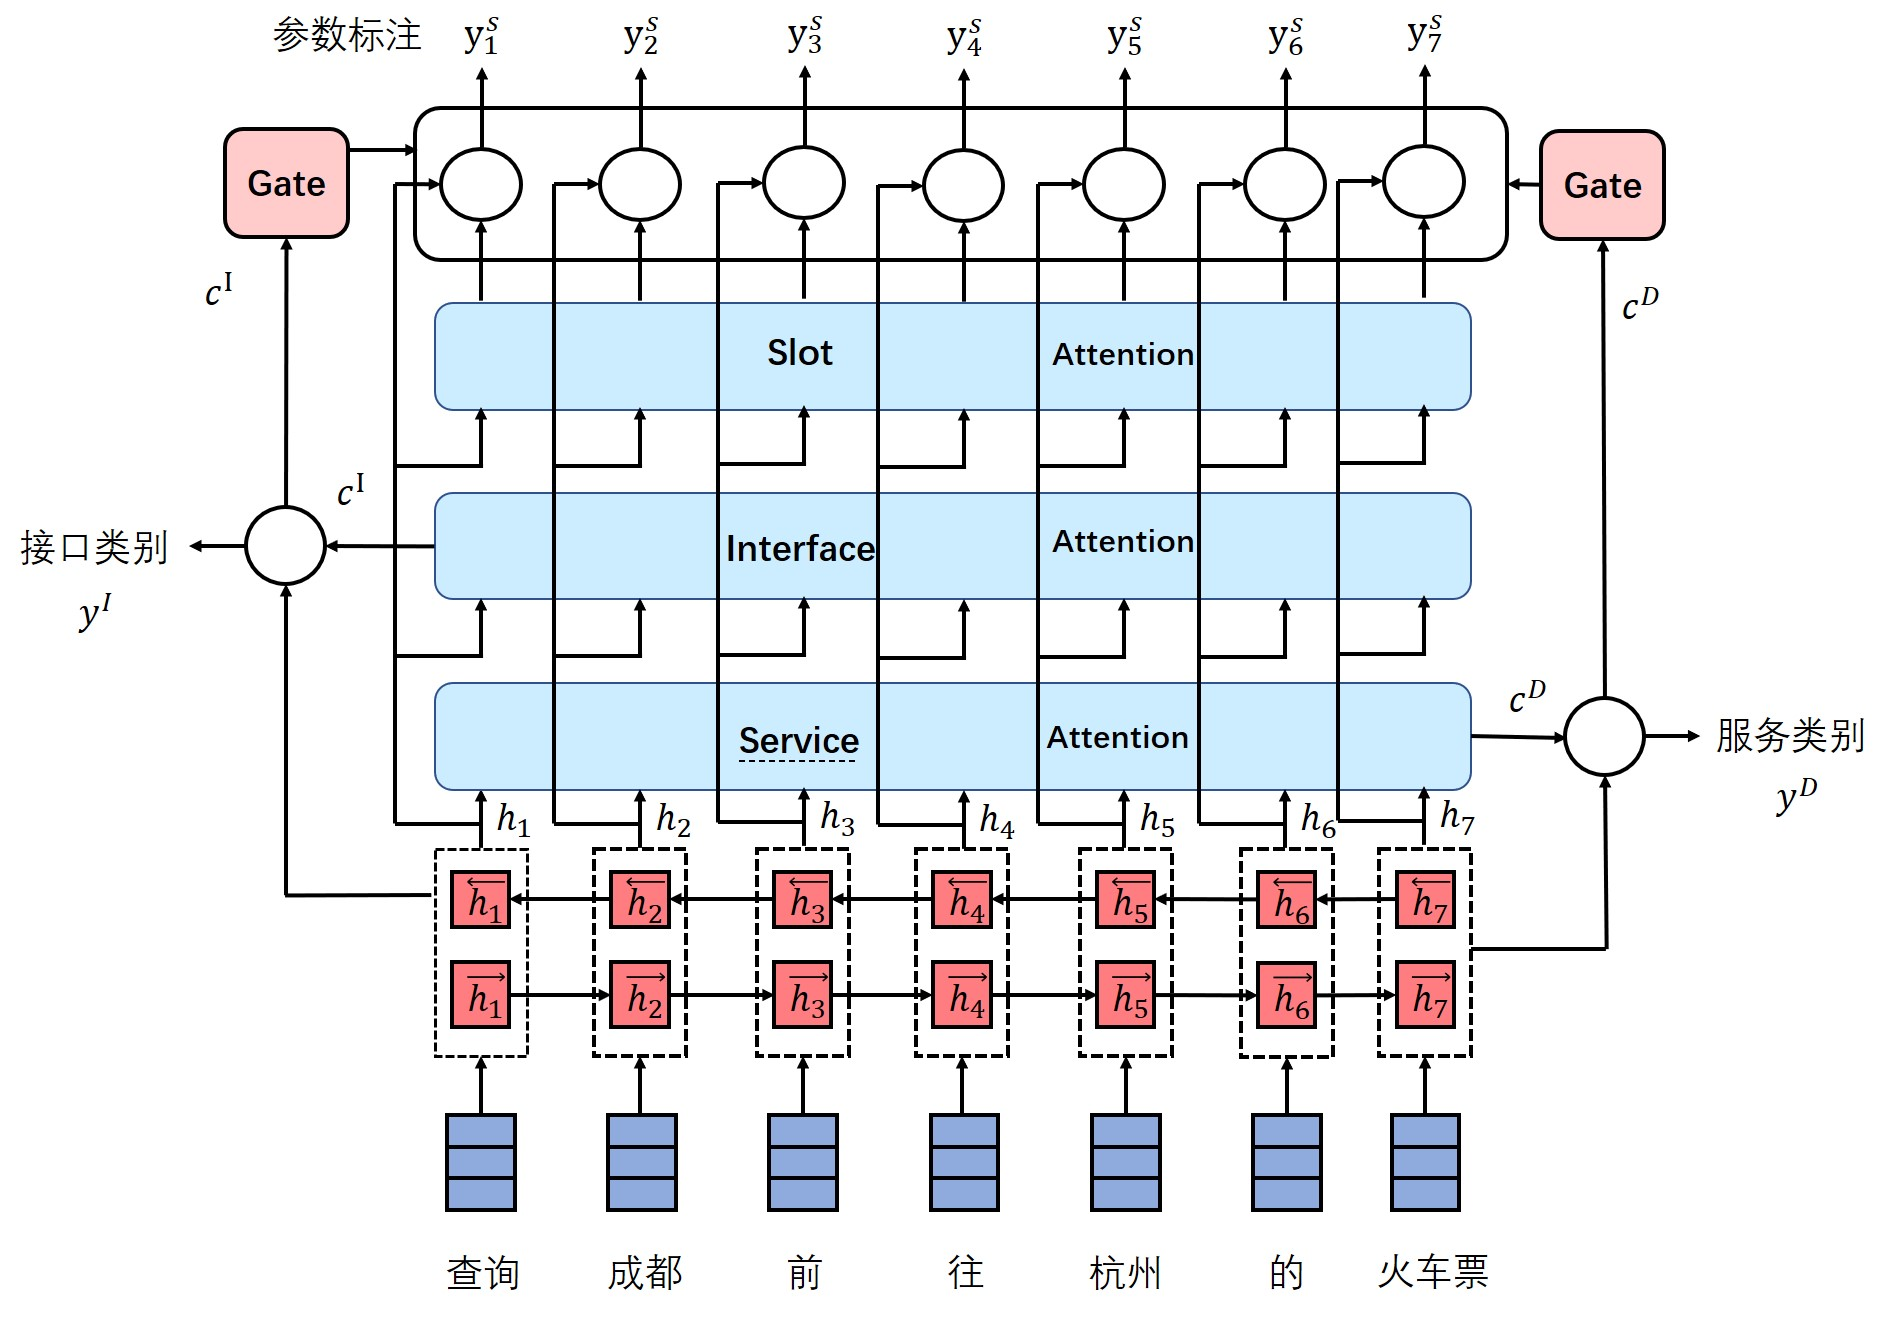
\includegraphics[width=17cm]{./images/lianhe.jpg}
    \caption{单向联合识别模型}
    \label{fig:lianhe1}
  \end{figure}

如图\ref{fig:lianhe}所示,是我们选择的联合识别模型。我们假设输入的词序列是x=[$x_{1}$,$x_{2}$,\dots,$x_{T}$],$x_{i}$经过双向LSTM处理后
得到的结果是$\overleftarrow{\mathbf{h}}_{i}$和$\overrightarrow{\mathbf{h}}_{i}$,拼接以后在第i步得到的结果是$\mathbf{h}_{i}=[\overrightarrow{\mathbf{h}}_{i} ;\overleftarrow{\mathbf{h}}_{i}]$。
1)三个attention层的计算方式

我们在联合模型中共设置了三层注意力机制,分别用于对应服务分类、接口分类与参数填充,三者的attention原理相同,只是会训练各自的参数,因此可以合并介绍。
设BLSTM得到的隐层向量序列为$h_{1}$,$h_{2}$,\dots,$h_{T}$,我们引入上下文向量${c}_{i}$来表示经过attention权重$α_{i,j}$和处理后的BLSTM隐层向量,
具体的${c}_{i}^{D}$,${c}_{i}^{I}$,${c}_{i}^{S}$分别表示用于服务分类、接口分类与参数填充任务的上下文向量:
\begin{equation}
    \mathbf{c}_{i}=\sum_{j=1}^{T} \alpha_{i, j} \mathbf{h}_{j}
  \end{equation}
  其中$\alpha_{i, j}$也根据所在具体的attention层不同分为$\alpha_{i, j}^{D}$,$\alpha_{i, j}^{I}$,$\alpha_{i, j}^{S}$,计算公式如下:
  \begin{equation}
    \alpha_{t, j}=\frac{\exp \left(\operatorname{score}\left(\mathbf{h}_{i}, \mathbf{h}_{j}\right)\right)}{\sum_{k} \exp \left(\operatorname{score}\left(\mathbf{h}_{i}, \mathbf{x}_{k}\right)\right)}
    \end{equation}
    \begin{equation}
      \operatorname{score}(\mathbf{h}_{i}, \mathbf{h}_{j}))=\tanh \left(\mathbf{W}\left[\mathbf{h}_{i} ; \mathbf{h}_{j}\right]\right)
    \end{equation}
显然这里的$\mathbf{W}$可由任务具体分为$\mathbf{W}_D$,$\mathbf{W}_I$,$\mathbf{W}_S$

2)服务分类

我们以1)中计算服务分类上下文向量的方法可以得到${c}_{i}^{D}$,再从BLSTM中取$\overleftarrow{\mathbf{h}}_{1}$和$\overrightarrow{\mathbf{h}}_{T}$,
$c^{D}$表示所有步骤得到的$c_i^{D}$的均值,服务的分类预测可由下式得到:
\begin{equation}
    y^{D}=\operatorname{softmax}\left(W^{D}\left(\overleftarrow{\mathbf{h}}_{1}+\overrightarrow{\mathbf{h}}_{T}+c^{D}\right)\right)
  \end{equation}
  \begin{equation}
    c^{D}=\frac{\sum_{i=1}^{T} c_i^{D}}{T}
  \end{equation}
3)接口分类

  我们以1)中计算接口分类上下文向量的方法可以得到${c}_{i}^{D}$,再从BLSTM中取$\overleftarrow{\mathbf{h}}_{1}$和$\overrightarrow{\mathbf{h}}_{T}$,
  $c^{I}$表示所有步骤得到的$c_i^{I}$的均值,服务的分类预测可由下式得到:
  \begin{equation}
      y^{I}=\operatorname{softmax}\left(W^{I}\left(\overleftarrow{\mathbf{h}}_{1}+\overrightarrow{\mathbf{h}}_{T}+c^{I}\right)\right)
    \end{equation} 
    \begin{equation}
        c^{I}=\frac{\sum_{i=1}^{T} c_i^{I}}{T}
      \end{equation}

      \begin{figure}[htbp]
        \centering
        
\includegraphics[scale=0.5]{./images/gate.jpg}
        \caption{gate结构}
        \label{fig:gate}
      \end{figure}

4)参数填充

如图\ref{fig:lianhe}中的gate,我们引入槽填充的控制门利用服务类型上下文向量${c}_{i}^{D}$和接口类型上下文向量${c}_{i}^{I}$来建立服务、接口与参数填充的关系
期望提高槽填充的准确率。${c}^{D}$,${c}^{I}$,${c}_{i}^{S}$会在每一个步长传入gate\ref{fig:gate}门结构中计算:
\begin{equation}
    g=\sum v \cdot \tanh (c_{i}^{S}+W_D \cdot c^{D}+W_I \cdot c^{I})
  \end{equation}
其中$\mathbf{v},\mathbf{W}_D,\mathbf{W}_I$是可训练的参数,数值g可以被看作联合上下文向量${c}^{D}$,${c}^{I}$,${c}_{i}^{S}$计算得到的权值,
较大的g表示slot上下文向量和D、I上下文向量注意到了输入序列的同一部分,可以推断出该语义槽和服务、接口之间的相关性更强,更有可能为我们需要提取的参数。
最终第i个词的标签类别信息可由下式计算得出:
\begin{equation}
    y_{i}^{S}=\operatorname{softmax}\left(W_{h y}^{S}\left(h_{i}+c_{i}^{S} \cdot g\right)\right)
  \end{equation}

5)联合目标函数
为了同时完成服务分类、接口分类与参数填充三项任务,需要建立联合损失函数,假设$y^D,y^I,y^S$表示正确的类别与标注,我们的目标
便是使在输入为$\mathbf{x}$的条件下概率$p\left(y^{S}, y^{I},y^{D} \mid \mathbf{x}\right)$最大:
\begin{equation}
    \begin{array}{l}
        p\left(y^{S}, y^{I},y^{D} \mid \mathbf{x}\right) \\
        =p\left(y^{D} \mid \mathbf{x}\right) p\left(y^{I} \mid \mathbf{x}\right) \prod_{t=1}^{T} p\left(y_{t}^{S} \mid \mathbf{x}\right) \\
        =p(y^{D} \mid x_{1}, \ldots, x_{T}) p(y^{I} \mid x_{1}, \ldots, x_{T}) \prod_{t=1}^{T} p(y_{t}^{S} \mid x_{1}, \ldots, x_{T})
        \end{array}
    \end{equation}

\subsection{交互式联合}
上一个的模型完成了从各任务独自建模到服务分类、接口分类向参数填充传递信息流的转换,但我们希望在任务与任务之间能够建立双向的信息交互。
直观的讲,如果用户的意图是调用平台内部的火车票查询服务,他输入的语句更可能出现诸如起始终点城市,日期等语义槽;反之,如果一句话中包含了
出发的起始,目的地和日期,那用户的意图更可能是调用行程相关的服务。因此,考虑到两个任务之间的交叉影响十分重要。在本模型中,核心组件是
交互影响模块,用于对两个任务之间的关系建模,旨在考虑两个任务的交叉影响以及相互促进。具体来说,在交互影响模块中,
我们首先在服务、接口和参数填充分别应用注意力机制,以捕获初始的显式向量表示形式,从而提取三个任务的语义信息。
其次,将明确的服务、接口和参数填充表示形式馈入一个共同交互的注意层,以进行相互交互。
参考transformer的设计,将服务分类向量视为查询$Q_D$,参数填充向量视为键$K_S$以及值$K_S$,以获取可感知服务分类信息的参数填充向量表示;
接口分类向量视为键$K_I$以及值$K_I$,以获取可感知服务分类信息的接口向量表示。
将接口分类向量视为查询$Q_I$,参数填充向量视为键$K_S$以及值$K_S$,以获取可感知接口分类信息的参数填充向量表示;
服务分类向量视为键$K_D$以及值$K_D$,以获取可感知接口分类信息的服务向量表示。
将参数填充向量视为查询$Q_D$,服务分类向量视为键$K_S$以及值$K_S$,以获取可感知参数填充信息的服务分类向量表示;
接口分类向量视为键$K_I$以及值$K_I$,以获取可感知参数填充信息的接口向量表示。
基于此操作,可以建立多个任务之间的显示连接,背后的原理通过协同互动的注意力机制获取相应的相互信息。

\begin{figure}[htbp]
  \centering
  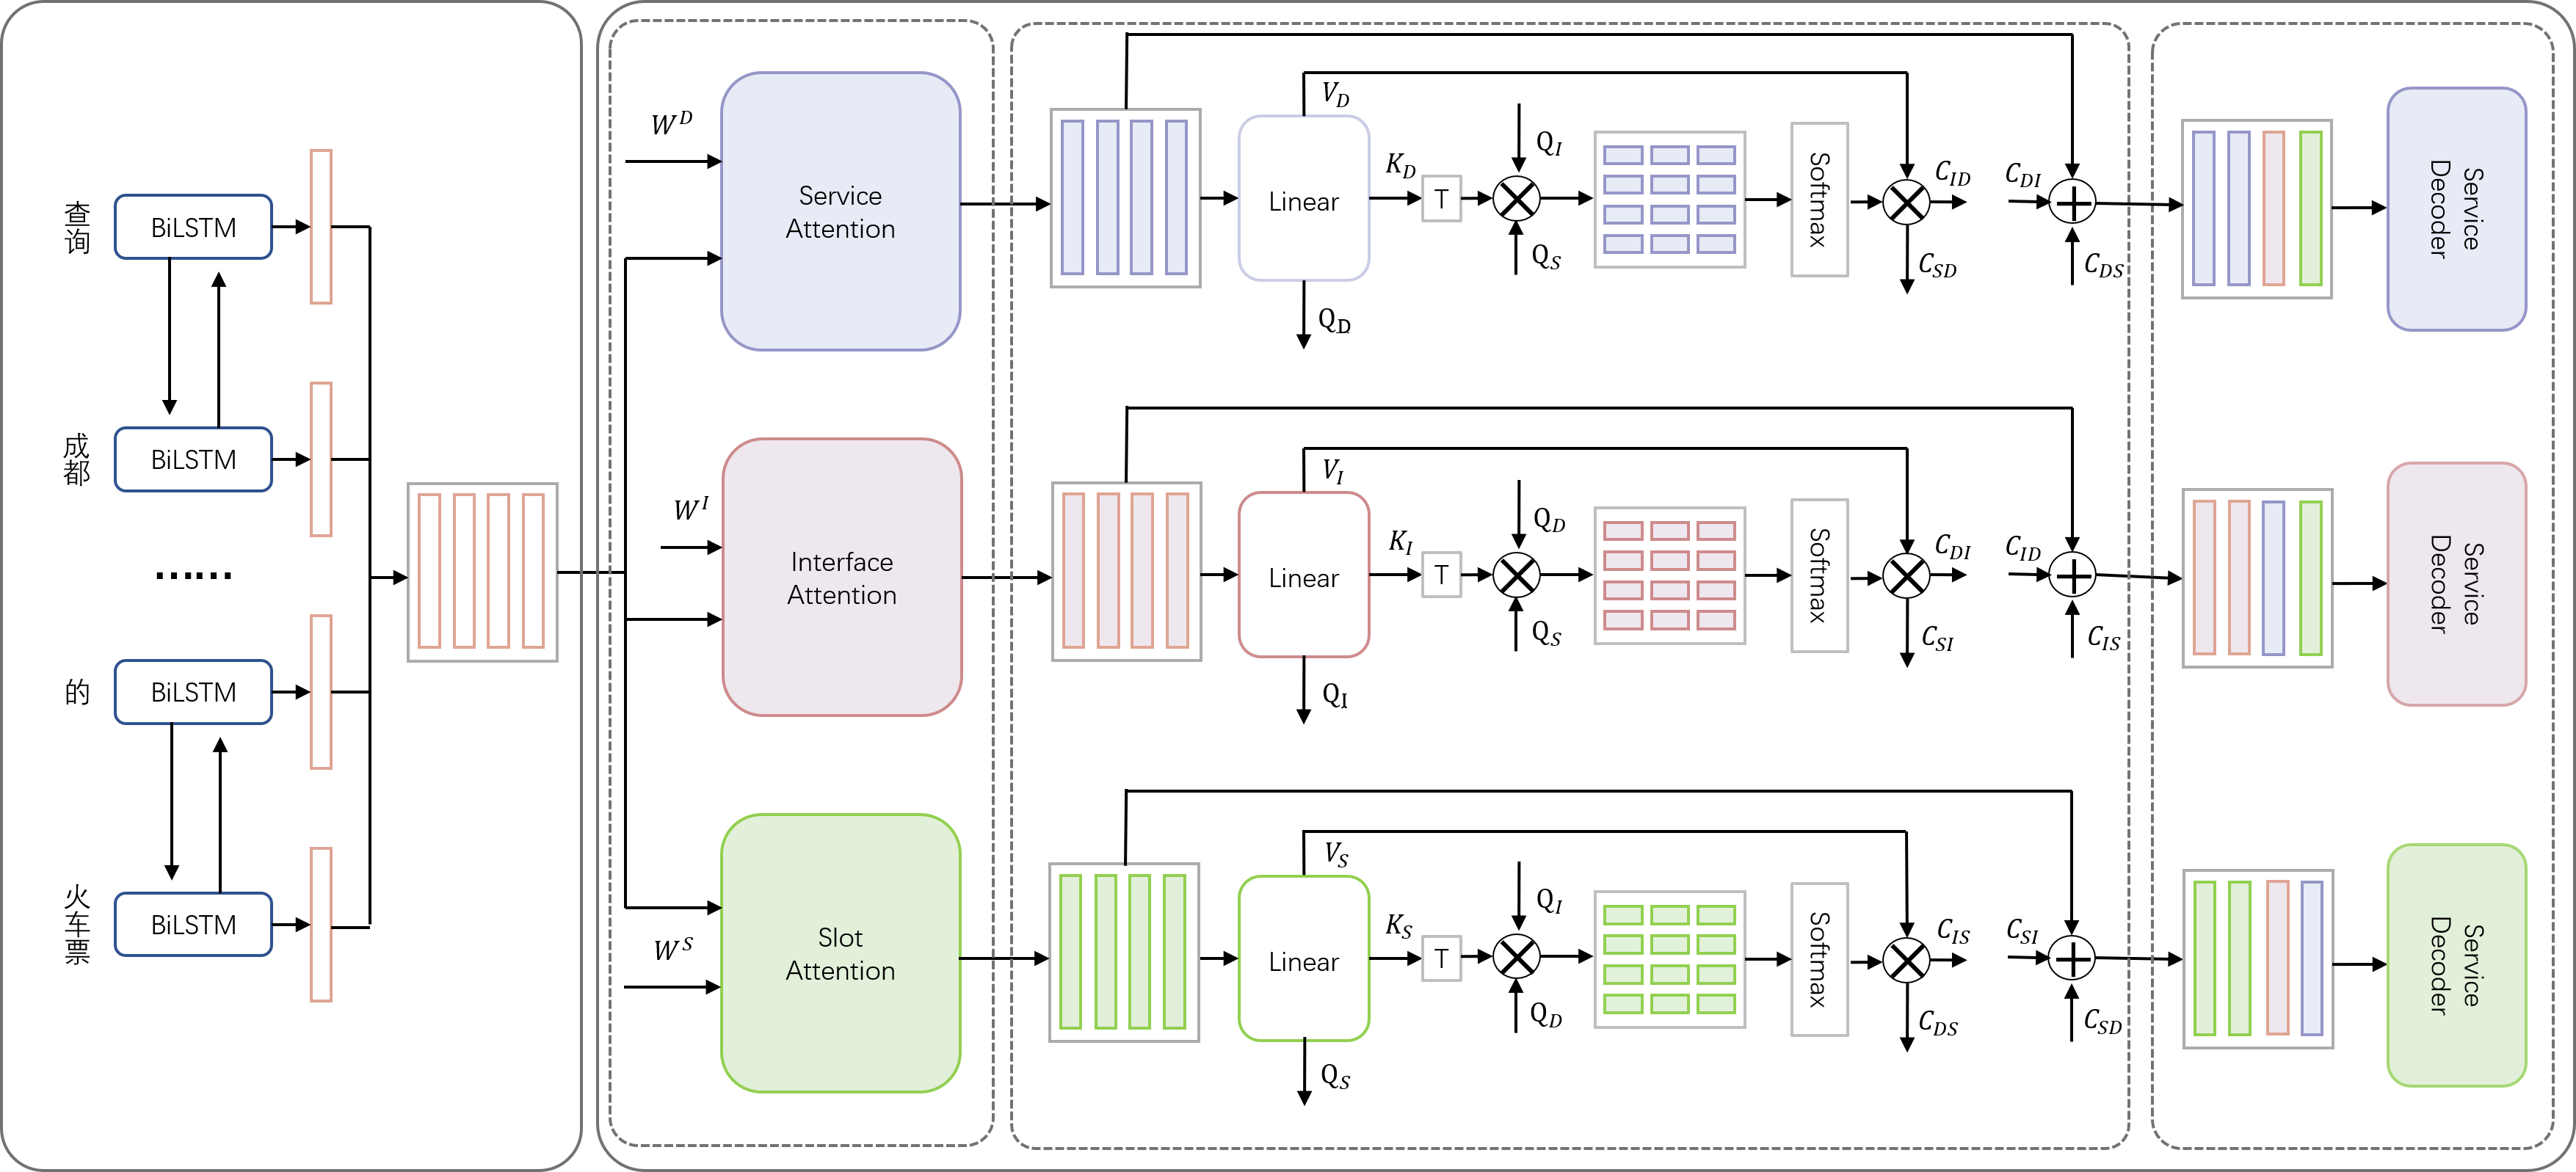
\includegraphics[width=18cm]{./images/co-interactive.jpg}
  \caption{交互式联合识别模型}
  \label{fig:lianhe2}
\end{figure}

交互式联合识别模型的结构如图\ref{fig:lianhe2}所示,主要包含的部分是:共享编码层,注意力层,交互层,独立解码层,接下将分别介绍:
1)共享编码层

我们使用双向LSTM作为编码器,设输入词序列是x=[$x_{1}$,$x_{2}$,\dots,$x_{n}$],$x_{i}$(n为词的数量)经过双向LSTM处理后
得到的结果是$\overleftarrow{\mathbf{h}}_{i}$和$\overrightarrow{\mathbf{h}}_{i}$,拼接以后在第i步得到的结果是$\mathbf{h}_{i}=[\overrightarrow{\mathbf{h}}_{i} ;\overleftarrow{\mathbf{h}}_{i}]$,
编码后得到的矩阵为$\mathbf{H}$=[$h_{1}$,$h_{2}$,\dots,$h_{n}$]

2)注意力层
我们为服务分类、接口分类向参数填充三个任务分别引入了注意力机制,将注意力处理以后得到的向量作为相应任务的向量表示传入交互层。
三者的attention原理相同,只是会训练各自的参数,因此可以合并介绍。
我们引入上下文向量${c}_{i}$来表示经过attention权重$α_{i,j}$和处理后的BLSTM隐层向量:
\begin{equation}
    \mathbf{c}_{i}=\sum_{j=1}^{n} \alpha_{i, j} \mathbf{h}_{j}
  \end{equation}
  得到经过attention处理的句子矩阵表示$\mathbf{C}$=[$c_{1}$,$c_{2}$,\dots,$c_{n}$],其中$\alpha_{i, j}$也根据所在具体的attention层不同分为$\alpha_{i, j}^{D}$,$\alpha_{i, j}^{I}$,$\alpha_{i, j}^{S}$,计算公式如下:
  \begin{equation}
    \alpha_{t, j}=\frac{\exp \left(\operatorname{score}\left(\mathbf{h}_{i}, \mathbf{h}_{j}\right)\right)}{\sum_{k} \exp \left(\operatorname{score}\left(\mathbf{h}_{i}, \mathbf{x}_{k}\right)\right)}
    \end{equation}
    \begin{equation}
      \operatorname{score}(\mathbf{h}_{i}, \mathbf{h}_{j}))=\tanh \left(\mathbf{W}\left[\mathbf{h}_{i} ; \mathbf{h}_{j}\right]\right)
    \end{equation}
显然这里的$\mathbf{W}$可由任务具体分为$\mathbf{W}_D$,$\mathbf{W}_I$,$\mathbf{W}_S$,最后我们将H矩阵与attention处理的C矩阵相加:
\begin{equation}
  \mathbf{H}=\mathbf{H}+\mathbf{C}
\end{equation}
这里H会根据训练时参数的不同分为三类$\mathbf{H}_{D},\mathbf{H}_{I},\mathbf{H}_{S}$,分别表示服务分类、接口分类向参数填充三项任务语义相关的显示的矩阵表示。

3)交互层
本层是多个任务的信息流建立信息交换的核心层,上层共得到三个矩阵$\mathbf{H}_{D},\mathbf{H}_{I},\mathbf{H}_{S}$,他们是任务相关的独立的语义表示,本层主要目的
是在借助其他两项任务指导下更新当前任务对应的H矩阵,达到交互信息流的目的,提高模型准确率。
首先我们将$\mathbf{H}_{D},\mathbf{H}_{I},\mathbf{H}_{S}$分别做三组线性变换得到矩阵($\mathbf{Q}_{D},\mathbf{Q}_{I},\mathbf{Q}_{S}$),
($\mathbf{K}_{D},\mathbf{K}_{I},\mathbf{K}_{S}$),($\mathbf{V}_{D},\mathbf{V}_{I},\mathbf{V}_{S}$),之后的计算借鉴attention思想。
对于服务分类任务,将$\mathbf{Q}_{D}$最为queries,$\mathbf{K}_{I}$作为keys和$\mathbf{V}_{I}$作为values,$\mathbf{K}_{S}$作为keys和$\mathbf{V}_{S}$作为values,做以下处理来达到信息的交互:
\begin{equation}
  \mathbf{C}_{\mathbf{DI}}=\operatorname{softmax}\left(\frac{\mathbf{Q}_{\mathbf{D}} \mathbf{K}_{\mathbf{I}}^{\top}}{\sqrt{d_{k}}}\right) \mathbf{V}_{\mathbf{I}}\\
\end{equation}
\begin{equation}  
\mathbf{C}_{\mathbf{DS}}=\operatorname{softmax}\left(\frac{\mathbf{Q}_{\mathbf{D}} \mathbf{K}_{\mathbf{S}}^{\top}}{\sqrt{d_{k}}}\right) \mathbf{V}_{\mathbf{S}}\\
\end{equation}
\begin{equation}  
\mathbf{H}_\mathbf{D}=\mathbf{H}_\mathbf{D}+\mathbf{C}_{\mathbf{DI}}+\mathbf{C}_{\mathbf{DS}}
\end{equation}
对于接口分类任务,将$\mathbf{Q}_{I}$最为queries,$\mathbf{K}_{D}$作为keys和$\mathbf{V}_{D}$values,$\mathbf{K}_{S}$作为keys和$\mathbf{V}_{S}$values,做以下处理来达到信息的交互:
\begin{equation}
  \mathbf{C}_{\mathbf{ID}}=\operatorname{softmax}\left(\frac{\mathbf{Q}_{\mathbf{I}} \mathbf{K}_{\mathbf{D}}^{\top}}{\sqrt{d_{k}}}\right) \mathbf{V}_{\mathbf{D}}\\
\end{equation}
\begin{equation}
  \mathbf{C}_{\mathbf{IS}}=\operatorname{softmax}\left(\frac{\mathbf{Q}_{\mathbf{I}} \mathbf{K}_{\mathbf{S}}^{\top}}{\sqrt{d_{k}}}\right) \mathbf{V}_{\mathbf{S}}\\
\end{equation}
\begin{equation}
  \mathbf{H}_\mathbf{I}=\mathbf{H}_\mathbf{I}+\mathbf{C}_{\mathbf{ID}}+\mathbf{C}_{\mathbf{IS}}
\end{equation}
对于接口分类任务,将$\mathbf{Q}_{S}$最为queries,$\mathbf{K}_{D}$作为keys和$\mathbf{V}_{D}$values,$\mathbf{K}_{I}$作为keys和$\mathbf{V}_{I}$values,做以下处理来达到信息的交互:
\begin{equation}
  \mathbf{C}_{\mathbf{SD}}=\operatorname{softmax}\left(\frac{\mathbf{Q}_{\mathbf{S}} \mathbf{K}_{\mathbf{D}}^{\top}}{\sqrt{d_{k}}}\right) \mathbf{V}_{\mathbf{D}}\\
\end{equation}
\begin{equation}
  \mathbf{C}_{\mathbf{SI}}=\operatorname{softmax}\left(\frac{\mathbf{Q}_{\mathbf{S}} \mathbf{K}_{\mathbf{I}}^{\top}}{\sqrt{d_{k}}}\right) \mathbf{V}_{\mathbf{I}}\\
\end{equation}
\begin{equation}
  \mathbf{H}_\mathbf{S}=\mathbf{H}_\mathbf{S}+\mathbf{C}_{\mathbf{SD}}+\mathbf{C}_{\mathbf{SI}}
\end{equation}

其中$d_k$是Q,K矩阵的列数,即向量维度。我们认为经过上面计算更新过后的矩阵$\mathbf{H}_{D},\mathbf{H}_{I},\mathbf{H}_{S}$,包含了更丰富的语义信息,
实现了多任务之间信息的交互。

4)独立解码层

在经过共享的交互层以后,各任务拥有自己独立的解码层。
对于服务分类任务,我们使用上一章介绍的CNN的max-pooling方法,将$\mathbf{H}_{D}$经过max-pooling处理得到一个句子语义级表示的向量$\mathbf{M}_D$,
之后经过softmax函数:
\begin{equation}
  \mathbf{y}^{D}=\operatorname{softmax} (\mathbf{W}^{D}\mathbf{M}_D+b)
\end{equation}
\begin{equation}
  \mathbf{O}^{D}=\operatorname{argmax} (\mathbf{y}^{D})
\end{equation}
$\mathbf{y}^{D}$是输出的服务类别的分布,$\mathbf{O}^{D}$是预测的服务类别,$\mathbf{W}^{D}$和b都是训练的参数。
对于接口分类任务解码器也做同样的处理,使用CNN的max-pooling方法,将$\mathbf{H}_{D}$经过max-pooling处理得到一个句子语义级表示的向量$\mathbf{M}_I$,
之后经过softmax函数:
\begin{equation}
  \mathbf{y}^{I}=\operatorname{softmax} (\mathbf{W}^{I}\mathbf{M}_I+b)
\end{equation}
\begin{equation}
  \mathbf{O}^{I}=\operatorname{argmax} (\mathbf{y}^{I})
\end{equation}
$\mathbf{y}^{I}$是输出的服务类别的分布,$\mathbf{O}^{I}$是预测的服务类别,$\mathbf{W}^{I}$和b都是训练的参数。
对于参数提取即语义槽填充任务,为了更好的建模标签与标签之间的依赖性,我们在解码层加了CRF处理,如下式所示:
\begin{equation}
  \mathbf{O}_{\mathbf{S}} =\mathbf{W}^{\mathbf{S}} {\mathbf{H}}_{\mathbf{S}}+\mathbf{b}_{\mathbf{S}} 
\end{equation}
\begin{equation}
  P\left(\hat{\mathbf{y}} \mid \mathbf{O}_{\mathbf{S}}\right) =\frac{\sum_{i=1} \exp f\left(y_{i-1}, y_{i}, \mathbf{O}_{\mathbf{S}}\right)}{\sum_{y^{\prime}} \sum_{i=1} \exp f\left(y_{i-1}^{\prime}, y_{i}^{\prime}, \mathbf{O}_{\mathbf{S}}\right)}
  \end{equation}
  $f(y_{i-1}, y_{i}, \mathbf{O}_{\mathbf{S}})$表示从标签$y_{i-1}$到标签$y_{i}$的转移分数,以及标签$y_{i}$自身的得分。
同时我们采用联合损失函数的形式对三项任务一起训练,服务分类预测的交叉熵损失函数可记为:
\begin{equation}
\mathcal{L}_{1} \triangleq-\sum_{j=1}^{m} \hat{\mathbf{y}}^{j, \mathbf{D}} \log \left(\mathbf{y}^{j, \mathbf{D}}\right)
\end{equation}
同理,接口分类交叉熵损失函数可记为:
\begin{equation}
  \mathcal{L}_{2} \triangleq-\sum_{j=1}^{m} \hat{\mathbf{y}}^{j, \mathbf{I}} \log \left(\mathbf{y}^{j, \mathbf{I}}\right)
  \end{equation}
  参数语义槽填充交叉熵损失函数可记为:
  \begin{equation}
    \mathcal{L}_{3} \triangleq-\sum_{j=1}^{m} \sum_{i=1}^{n_{j}} \hat{\mathbf{y}}_{i}^{j, \mathbf{S}} \log \left(\mathbf{y}_{i}^{j, \mathbf{S}}\right)
  \end{equation}
  其中$\hat{\mathbf{y}}^{j, \mathbf{D}},\hat{\mathbf{y}}^{j, \mathbf{I}},\hat{\mathbf{y}}_{i}^{j, \mathbf{S}}$为真实值,m是训练的数据总量,联合损失函数
  可表示为:
  \begin{equation}
    \mathcal{L}_{\theta}=\alpha \mathcal{L}_{1}+\beta \mathcal{L}_{2}+(1-\alpha-\beta) \mathcal{L}_{3}
  \end{equation}
  其中$\alpha,\beta$为超参数。

\section{结合bert的模型}

大量研究表明,语言模型预训练对于学习通用语言表示很有用,作为最新的语言模型预训练模型,BERT在许多语言理解任务中均取得了惊人的成绩。
bert预训练模型的使用可以避免从头开始训练新模型,它通过利用大量非标注数据来学习语言的通用表示形式。

官方提供了不同参数的多版本bert供使用,本模型选择的是BERT-Base Chinese,
其中 L = 12, H = 768, A = 12 ,params的总量为 110 M 。具体来说, L = 12 指 Transformer 的层数为 12 层,
 H = 768 表示 Transformer 内部 包含 768 个隐含单元, A = 12 表示多头自制力机制中自注意力机制模型为 12 个\cite{devlin2018bert}。
 BERT依赖于Transformer(一种学习文本中单词之间的上下文关系的注意力机制),一个基本的Transformer由一个读取文本输入的编码器和一个对任务进行预测的解码器组成。
 由于BERT的目标是生成语言表示模型,因此只需要编码器部分即可。BERT编码器的输入是一系列token,这些token首先被转换为矢量,然后在神经网络中进行处理。
 但是在开始处理之前,BERT需要对输入进行处理并用一些额外的元数据修饰:

 1.令牌嵌入:在第一个句子的开头将[CLS]令牌添加到输入的单词令牌中,并在每个句子的末尾插入[SEP]令牌。

2.段嵌入:将指示句子A或句子B的标记添加到每个标记,这使编码器能够区分句子。

3.位置嵌入:将位置嵌入添加到每个标记,以指示其在句子中的位置。

因此,引入bert模型以后我们不再需要结巴分词工具,直接将句子按字向量序列输入bert模型编码,bert对输入的处理如图\ref{fig:bertInput}。
\begin{figure}[htbp]
  \centering
  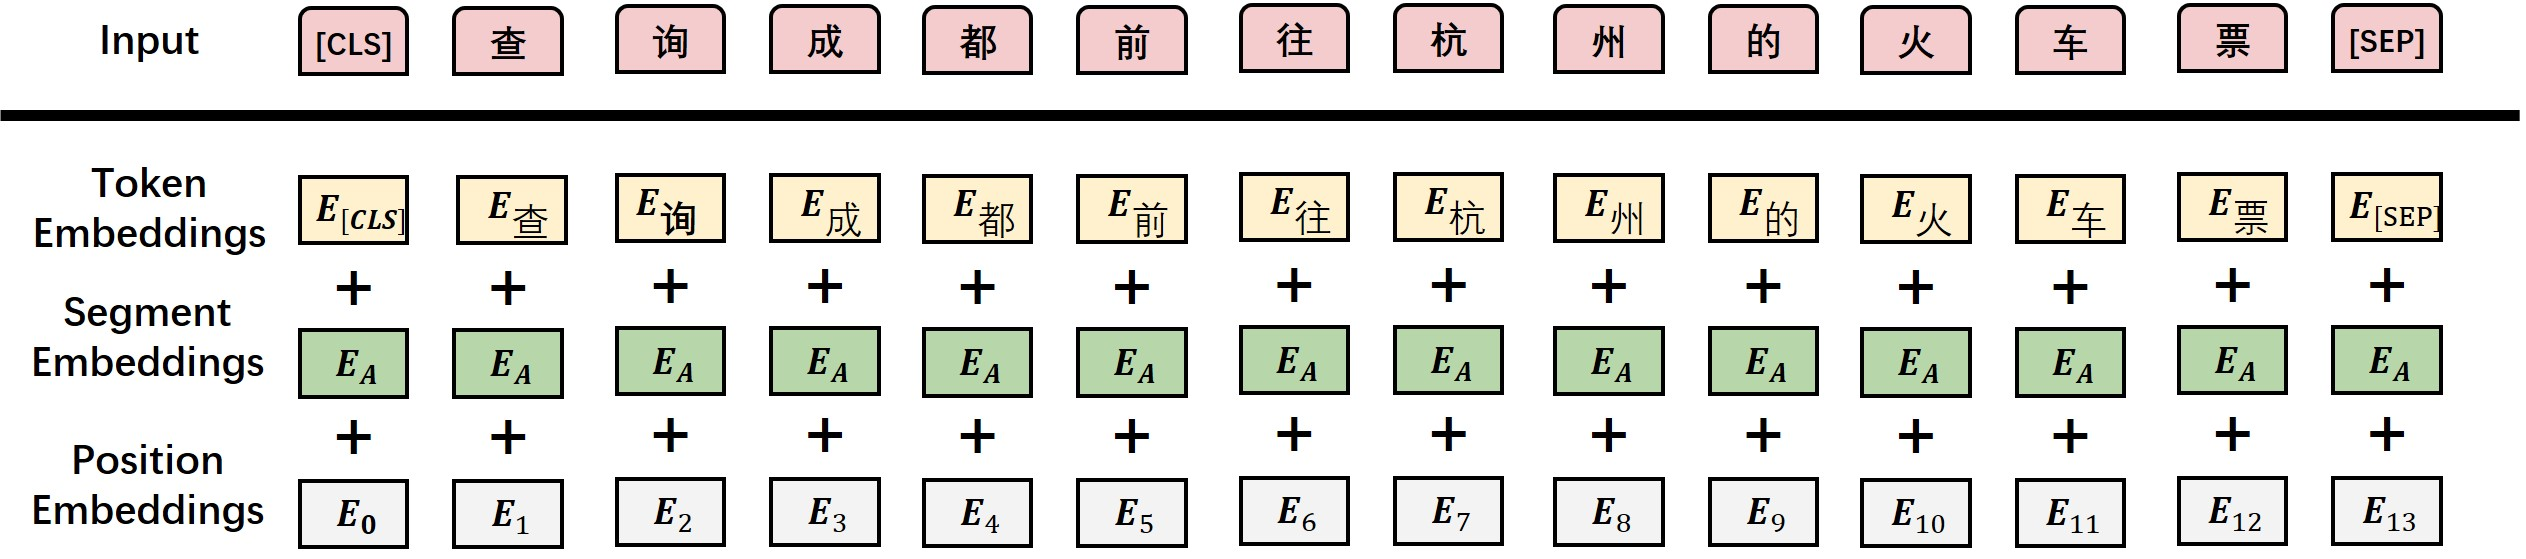
\includegraphics[width=18cm]{./images/bertInput.jpg}
  \caption{bert对输入的处理}
  \label{fig:bertInput}
\end{figure}

\subsection{引入bert的基础模型}
首先,我们提出最简版的bert-base模型,将服务分类、接口分类向参数填充三个任务利用联合损失函数隐式的建模,本模型主要起对照组的作用,
来验证引入bert是否能够解决NLU泛化能力差的问题,同时可以作为下一个模型的基准,模型架构如图\ref{fig:bert-base}所示。

\begin{figure}[htbp]
  \centering
  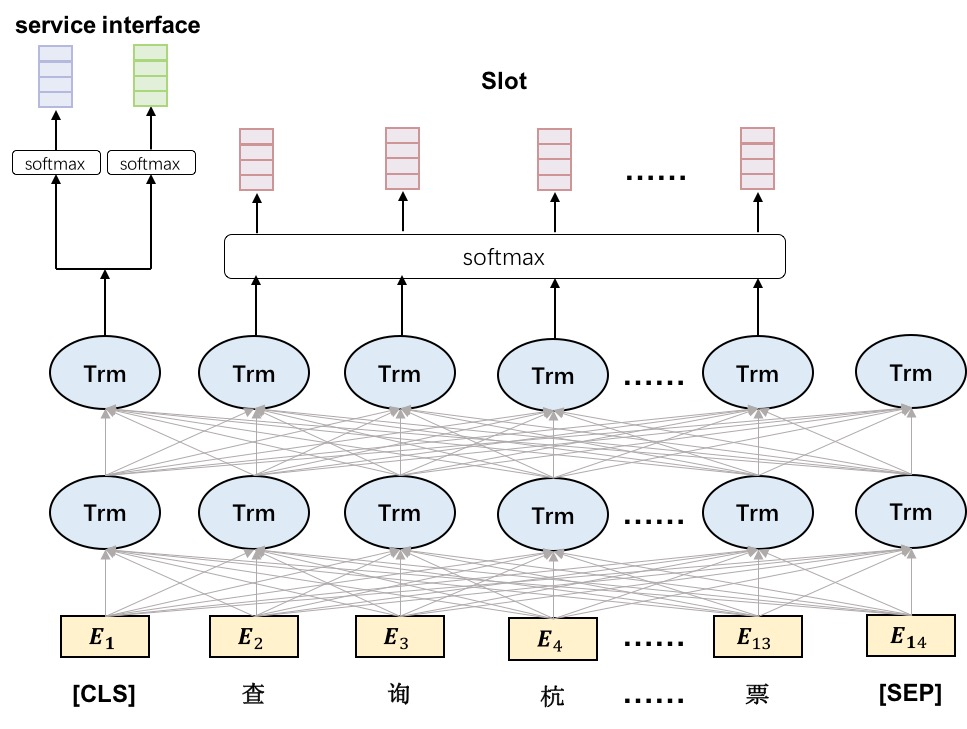
\includegraphics[width=16cm]{./images/bert-base.jpg}
  \caption{bert-base联合识别模型}
  \label{fig:bert-base}
\end{figure}

模型结构非常清晰,将用户语句按字向量序列输入bert模型编码,得到bert的输出$\mathbf{H}$=[$h_{1}$,$h_{2}$,\dots,$h_{n}$],
我们取bert输出的第一个向量,也就是特殊token([CLS])的隐藏状态作为两项分类任务的输入传给softmax层:
\begin{equation}
  y^{d}=\operatorname{softmax}\left(\mathbf{W}^{d} \boldsymbol{h}_{1}+\boldsymbol{b}^{d}\right)
\end{equation}
\begin{equation}
  y^{i}=\operatorname{softmax}\left(\mathbf{W}^{i} \boldsymbol{h}_{1}+\boldsymbol{b}^{i}\right)
\end{equation}
对于参数填充任务,将[$h_{2}$,\dots,$h_{n}$]隐层状态传入softmax层,以对插槽填充标签进行分类:
\begin{equation}
y_{n}^{s}=\operatorname{softmax}\left(\mathbf{W}^{s} \boldsymbol{h}_{n}+\boldsymbol{b}^{s}\right), n \in 2 \ldots N
\end{equation}
三项任务联合概率函数为:
\begin{equation}
  p\left(y^{d},y^{i}, y^{s} \mid \boldsymbol{x}\right)=p\left(y^{d} \mid \boldsymbol{x}\right) \left(y^{i} \mid \boldsymbol{x}\right) \prod_{n=1}^{N} p\left(y_{n}^{s} \mid \boldsymbol{x}\right)
  \end{equation}
  训练的目标是最大化正确标签的概率$p\left(y^{d},y^{i}, y^{s} \mid \boldsymbol{x}\right)$。

\subsection{引入bert的交互式联合识别模型}

为在交互式联合识别模型中引入bert,将interactive模型的共享编码器换成bert拼接在attention之前\ref{fig:bert-joint},模型其他结构与interactive模型
一致不再赘述,bert部分的参数采用fine-tuning的方式更新。
\begin{figure}[htbp]
  \centering
  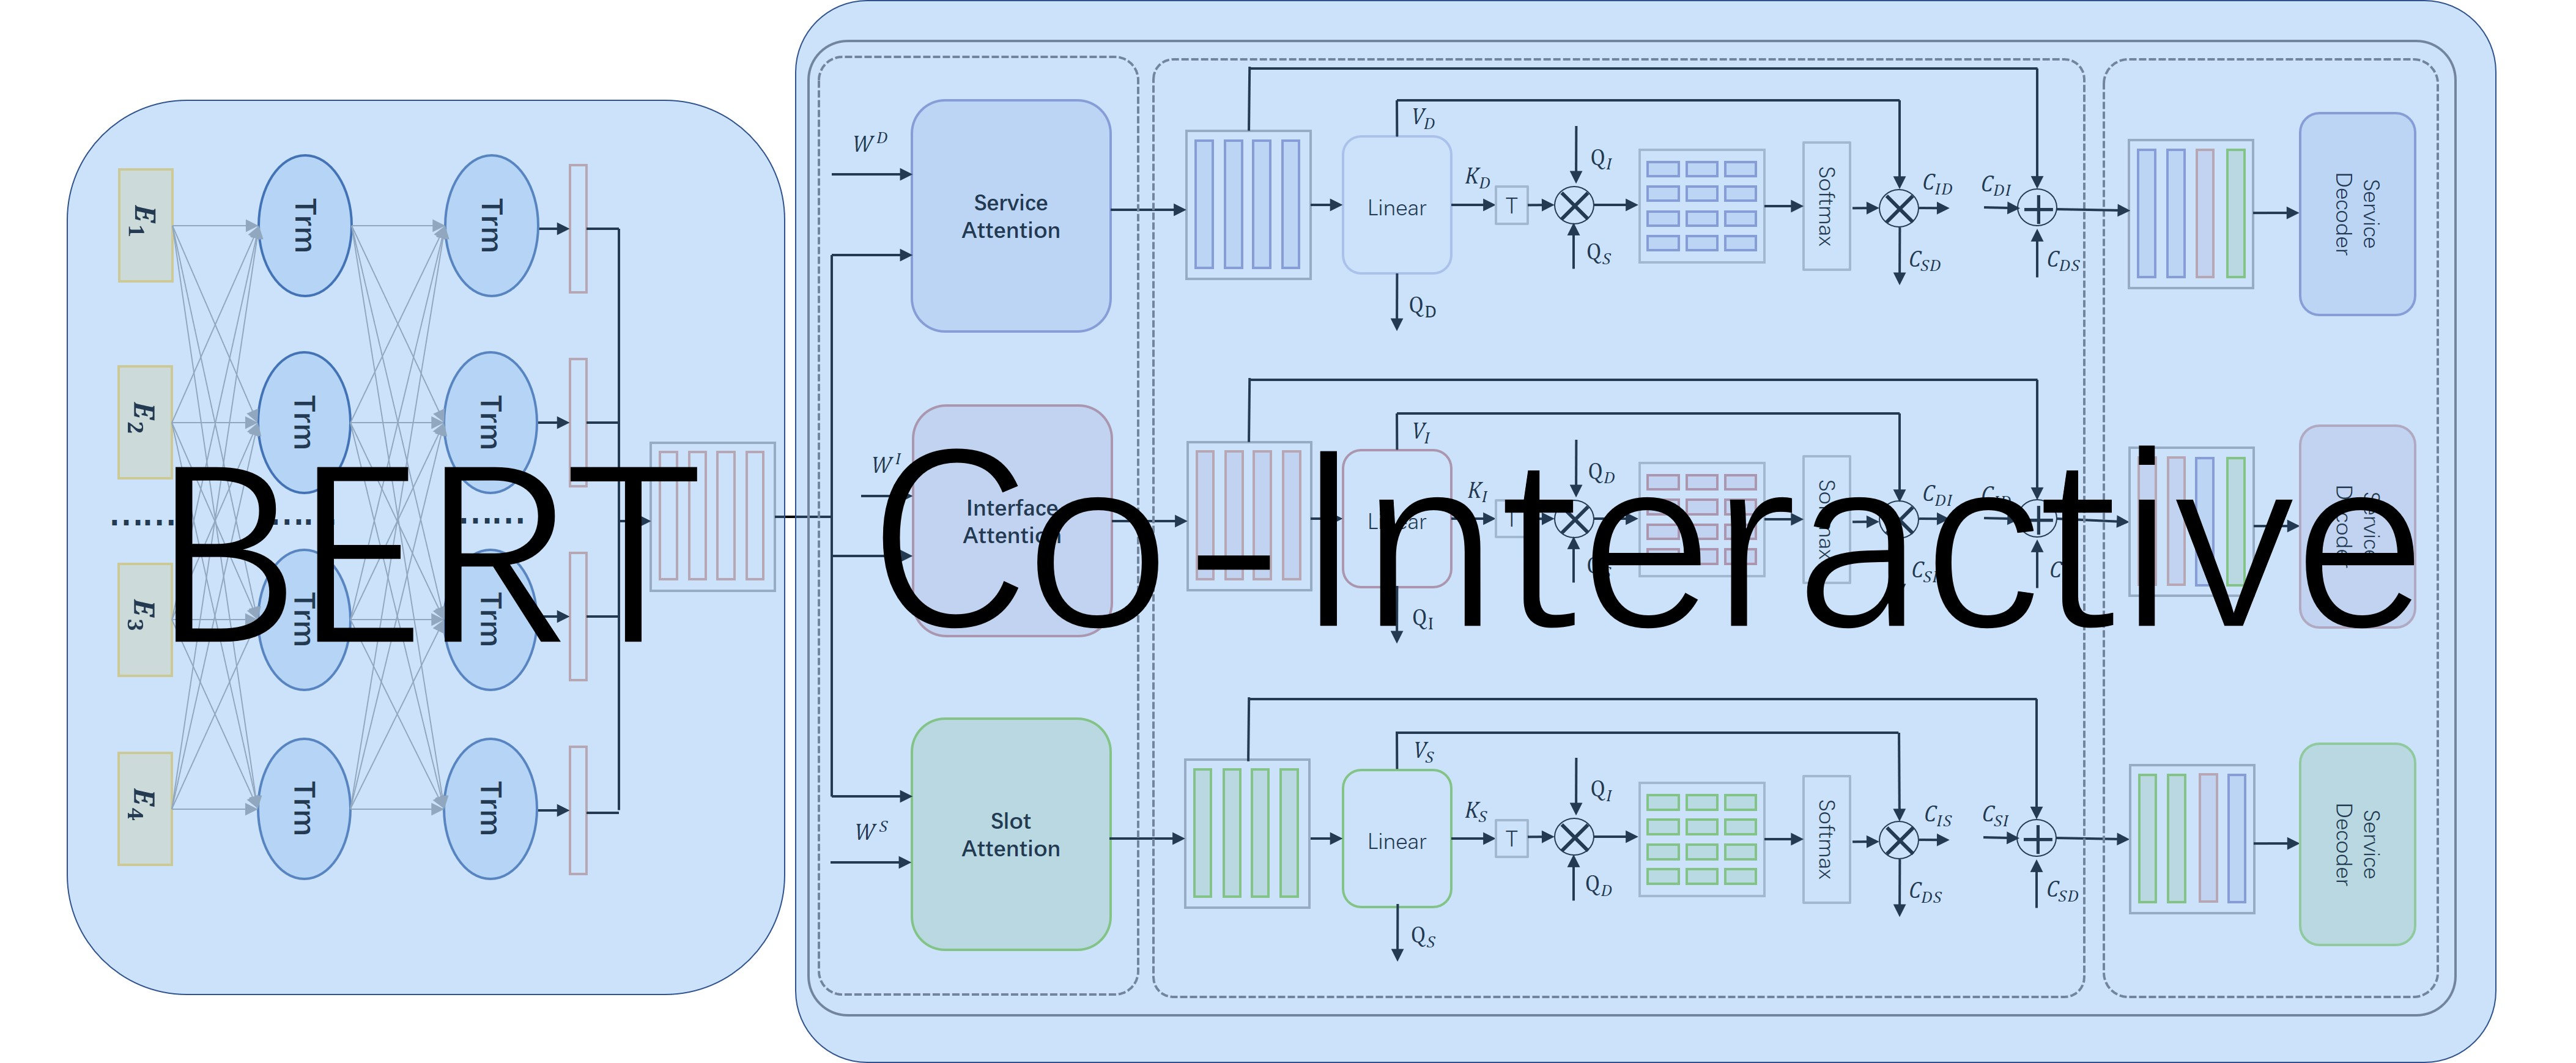
\includegraphics[width=16cm]{./images/bert-joint.jpg}
  \caption{引入bert交互式联合识别模型}
  \label{fig:bert-joint}
\end{figure}


% \section{结合ernie的模型}

